\appendix


\Large \textbf{Appendices}
\normalsize

\section{Group Axioms}\label{sec:group_axioms}


For a set of transformations $G$ to be a group under the operation $\cdot$, these four axioms must hold:

\begin{enumerate}
    \item \textit{Closure}: The product of any two elements of the group is also an element of the group, i.e., for all $g_1, g_2 \in G$, $g_1g_2 \in G$.
    \item \textit{Associativity}: The grouping of elements under the operation does not change the outcome, so long as the order of elements is preserved, i.e., $(g_1g_2)g_3 = g_1(g_2g_3)$.
    \item \textit{Identity}: There exists a ``do-nothing'' \textit{identity} element $e$ that such that the product of $e$ with any other element $g$ returns $g$, i.e., $ge = eg = g$ for all $g \in G$.
    \item \textit{Inverse}: For every element $g$, there exists an \textit{inverse} element $g^{-1}$  such that the product of $g$ and $g^{-1}$ returns the identity, i.e. $gg^{-1} = g^{-1}g = e$.
\end{enumerate}


\section{The Case of Steerable $G$-CNNs}\label{app:steerable}

We consider the framework of Steerable $G$-CNNs defined in \cite{cohen2016steerable}. Consider a group $G$ that is the semi-direct product $G=\mathbb{Z}_2 \ltimes H$ of the group of translations $\mathbb{Z}_2$ and a group $H$ of transformations that fixes the origin $0 \in \mathbb{Z}_2$. Consider the feature map $\Theta: \mathbb{Z}_2 \rightarrow \mathbb{R}^K$ that is the output of a steerable $G$-CNN. Here, $\Theta$ is a field that transforms according to a representation $\pi$ induced by a representation $\rho$ of $H$ on the fiber $R^K$.

The $G$-TC can be defined on $\Theta$ by replacing the regular representation by the induced representation. Specifically, replace any $\Theta(g)$, i.e. the scalar value of the feature map at group element $g$ by $\pi(g)(\Theta)(x)$, i.e., the vector value of the feature map at $x$ after a group element $g$ has acted on it via the representation $\pi$ :
$$
\tau_\Theta (g_1, g_2) =\int_G \pi(g)(\Theta)(x)^{\dagger} \cdot \pi\left(g_1 g\right)(\Theta)(x) \cdot \pi\left(g_2 g\right)(\Theta)(x) d g.
$$

Instead of computing the $G$-TC for each scalar coordinate $k$ of $\Theta$ as in the main text, we directly compute it as a vector. The formulation does not depend on the choice of $x$ by homogeneity of the domain $\mathbb{Z}_2$ for the group $G$. Importantly, this $G$-TC is invariant to the action of the induced representation, see Appendix~\ref{sec:g-tc-invariance}.




\section{The $G$-Triple Correlation: Concrete Examples}
\label{app:tc-examples}

We show how to compute the $G$-Triple Correlation ($G$-TC) on three concrete groups.
We start with the $G$-TC for the group $\mathbb{R}^2$ of 2D translations.

\begin{example}
Consider the group of 2D translations $G = (\mathbb{R}^2, +)$ with the addition as the group law. Consider a signal $\Theta$ that is a real function defined over $\mathbb{R}^2$ and can therefore be identified with an image. For any $x_1, x_2 \in \mathbb{R}^2$, the $G$-TC is given by:
\begin{equation}
    \tau_\Theta(x_1, x_2)
        = \int_{x \in \mathbb{R}^2} \Theta(x) \Theta\left(x +  x_1\right) \Theta\left(x +  x_2\right)dx.
\end{equation}
\end{example}

Next, we consider the special orthogonal group $SO(2)$ of 2D rotations.


\begin{example}
Consider the group of 2D rotations $G = (SO(2), \cdot )$ where $SO(2)$ is parameterized by $[0, 2\pi]$ and the composition of rotations $\cdot $ is the addition of angles modulo $2\pi$:
\begin{equation}
    \theta_1 \cdot \theta_2
    \equiv
    \theta_1 + \theta_2 [2\pi].
\end{equation}
For a real signal $\Theta$ defined over $G$, we have:
\begin{equation}
    \tau_\Theta(\theta_1, \theta_2)
        = \int_{\theta \in SO(2)} \Theta(\theta) \Theta\left(\theta + \theta_1\right) \Theta\left(\theta +  \theta_2\right)d\theta,
\end{equation}
    for any $\theta_1, \theta_2 \in SO(2)$ and the addition is taken modulo $2\pi$.
\end{example}

Finally, we compute the $G$-TC for the special euclidean group $SE(2)$ of 2D rotations and translations, i.e., of 2D rigid-body transformations.


\begin{example}
Consider the group of 2D rigid body transformations $G = SE(2) = (SO(2) \times \mathbb{R}^2, \cdot)$ equipped with the group composition law:
\begin{equation}
    (\theta_1, x_1) \cdot (\theta_2, x_2)
    \equiv
    (\theta_1 + \theta_2, R_{\theta_1}.x_2 + x_1),
\end{equation}
where $R_{\theta_1} = \begin{bmatrix}
    \cos \theta_1 & -\sin \theta_1 \\
    \sin \theta_1 & \cos \theta_1
\end{bmatrix}$ is the 2D rotation matrix associated with rotation $\theta_1$ and the addition of angles $\theta_1 + \theta_2$ is taken module $2\pi$.

For a real signal defined on $SE(2)$ we have:
\begin{align*}
    \tau_\Theta((\theta_1, x_1), (\theta_2, x_2))
        &= \int_{(\theta, x) \in SE(2)} \Theta(\theta, x) \Theta\left((\theta, x) \cdot (\theta_1, x_1)\right) \Theta\left((\theta, x) \cdot (\theta_2, x_2)\right)d\theta dx \\
        &= \int_{(\theta, x) \in SE(2)} \Theta(\theta, x) \Theta\left(\theta+\theta_1, R_\theta.x_1+x\right) \Theta\left(\theta +\theta_2, R_\theta.x_2 + x\right)d\theta dx,
\end{align*}
for any $\theta_1, \theta_2 \in SO(2)$ and $x_1, x_2 \in \mathbb{R}^2$.
\end{example}


\section{Invariance of the $G$-Triple Correlation}\label{sec:g-tc-invariance}

Consider a real signal $\Theta$ defined over a group $G$. The $G$-Triple Correlation is invariant to group actions on the domain of the signal $\Theta$ as shown in~\cite{KakaralaTriple}.

\begin{proposition}
    Consider two real signals $\Theta_1, \Theta_2$ defined over a group $G$. If there exists $h \in G$ such that one signal is obtained from the other by a group action, i.e., $\Theta_2 = \action_h[\Theta_1]$, then $\tau_{\Theta_1} = \tau_{\Theta_2}$.
\end{proposition}

We recall the proof of \cite{KakaralaTriple} below.

\begin{proof}
Consider two real signals $\Theta_1, \Theta_2$ defined over a group $G$, such that $\Theta_2 = L_h[\Theta_1]$ for a group action $L_h$ of group element $h$. We show that this implies that $\tau_{\Theta_1} = \tau_{\Theta_2}$.

Taking $g_1, g_2 \in G$, we have:
\begin{align*}
    \tau_{\Theta_2}(g_1, g_2)
        &= \int_{g \in G}
            \Theta_2(g) \Theta_2\left(gg_1\right) \Theta_2\left(gg_2\right) dg  \\
        &= \int_{g \in G}
            L_h[\Theta_1](g) L_h[\Theta_1]\left(gg_1\right) L_h[\Theta_1]\left(gg_2\right) dg  \\
        &= \int_{g \in G}
            \Theta_1(hg) \Theta_1\left(hgg_1\right) \Theta_1\left(hgg_2\right) dg  \\
        &= \int_{g \in G}
            \Theta_1(g) \Theta_1\left(gg_1\right) \Theta_1\left(gg_2\right) dg \\
        &=  \tau_{\Theta_1}(g_1, g_2).
\end{align*}
where we use the change of variable $hg \rightarrow g$.

This proves the invariance of the $G$-TC with respect to group actions on the signals.
\end{proof}

\section{Symmetries of the $G$-Triple Correlation}\label{app:symmetries}

The $G$-Triple Correlation ($G$-TC) enjoys some symmetries that we can leverage to avoid computing it for each pair of group elements (which would represent $|G|^2$ computations), hence making the feedforward pass more efficient.

These symmetries are given in the main text. We recall them here for completeness.

\begin{proposition}
Consider two transformations $g_1, g_2 \in G$. The $G$-Triple Correlation of a signal $\Theta$ has the following symmetry:
\begin{align*}
     (s1) \qquad T_\Theta(g_1, g_2) &= T_\Theta(g_2, g_1).
\end{align*}
If $G$ is commutative, the $G$-Triple Correlation of a real signal has the following additional symmetries:
\begin{align*}
     (s2) \qquad T_\Theta(g_1, g_2)
     = T_\Theta(g^{-1}_1, g_2g^{-1}_1)
     = T_\Theta(g_2g^{-1}_1, g^{-1}_1)
     = T_\Theta(g_1g^{-1}_2, g^{-1}_2)
     = T_\Theta(g^{-1}_2, g_1g^{-1}_2).
\end{align*}
\end{proposition}

Our proof extends the proof given in \cite{nikias1993signal} for the group of translations.

\begin{proof}
    Consider two transformations $g_1, g_2 \in G$.

    Symmetry (s1) relies on the fact that $\Theta(gg_2)$ and $\Theta(gg_1)$ are scalar values that commute:
    \begin{align*}
        T_\Theta(g_2, g_1)
            = \frac{1}{|G|} \sum_{g \in G} \Theta(g)\Theta(gg_2)\Theta(gg_1)
            = \frac{1}{|G|} \sum_{g \in G} \Theta(g)\Theta(gg_1)\Theta(gg_2)
            = T_\Theta(g_2, g_1).
    \end{align*}
    For symmetry (s2), we assume that $G$ is commutative.
    We prove the first equality:
    \begin{align*}
        T_\Theta(g^{-1}_1, g_2g^{-1}_1)
            &= \frac{1}{|G|} \sum_{g \in G} \Theta(g)\Theta(gg^{-1}_1)\Theta(gg_2g^{-1}_1) \\
            &= \frac{1}{|G|} \sum_{g' \in G} \Theta(g'g_1)\Theta(g')\Theta(g'g_1g_2g^{-1}_1)
                \quad \text{(with $g' = gg_1^{-1}$, i.e., $g=g'g_1$)} \\
            &= \frac{1}{|G|} \sum_{g' \in G} \Theta(g'g_1)\Theta(g')\Theta(g'g_2)
                \quad \text{($G$ commutative: $g_2 g^{-1}_1 = g^{-1}_1 g_2$)} \\
            &= \frac{1}{|G|} \sum_{g \in G} \Theta(gg_1)\Theta(g)\Theta(gg_2) \\
            &= \frac{1}{|G|} \sum_{g \in G} \Theta(g)\Theta(gg_1)\Theta(gg_2)
                \quad \text{($\Theta$ takes on real values that commute)}\\
            &= T_\Theta(g_2, g_1)
    \end{align*}
    The second equality of symmetry (s2) follows using (s1).
    The third and fourth equality of symmetry (s2) have the same proof.
\end{proof}

This result and its proof are also valid for the extension of the $G$-TC that we propose in Appendix~\ref{app:steerable}. They naturally emerge by replacing the regular representation by the induced representation in the proof above.

Specifically, consider a signal $\Theta_2=\pi\left(g_0\right)[\Theta_1]$ obtained from the action of $g_0$ on a signal $\Theta_1$. We want to show that $\tau_{\Theta_1} = \tau_{\Theta_2}$. The key ingredient of the proof is the change of variable within the integral $\int_{G^{\prime}}$, which follows the semi-direct product structure of $\mathrm{G}$ :
$$
h^{\prime}=h h_0 \text { and } t^{\prime}=\phi(h) t_0+t
$$
where $\phi(h)$ is a matrix representing h that acts on $\mathbb{Z}_2$ via matrix multiplication: e.g., a rotation matrix $R=\phi(r)$ in the case of $SE(n)$. This concludes the adaptation of the proof for the steerable case.



\section{Algorithmic Reduction}\label{app:reduction}

In this section, we show that we can reduce the complexity of the $G$-Triple Correlation of a real signal. This computational reduction requires that we consider, instead, the spectral dual of the $G$-TC, the bispectrum~\cite{kakarala2012bispectrum}. In what follows, we consider a signal $\Theta$ defined over a finite group $G$. The signal can be real or complex valued.

\subsection{Reduction for Commutative Groups}


Consider a commutative group $G$. The bispectrum for a signal $\Theta$ is defined over a pair of irreducible representations $\rho_1, \rho_2$ of the group $G$ as:
\begin{equation}
    \beta (\Theta)_{\rho_1, \rho_2} = \mathcal{F}(\Theta)_{\rho_1}^{\dagger}\mathcal{F}(\Theta)_{\rho_2}^{\dagger}\mathcal{F}(\Theta)_{\rho_1 \rho_2} \qquad \in \mathbb{C},
    \label{eqn:group-bs}
\end{equation}
where $\mathcal{F}(\Theta)$ is the Fourier transform of $\Theta$ that generalizes the classical Fourier transformation to signals defined over a group. We note that, in group theory, the irreducible representations (irreps) of commutative groups map to scalar values. Hence, the bispectrum is a complex scalar in this case.

For a discrete commutative group, the number of irreps is equal to the size of the group. \cite{KondorThesis} proved that, for cyclic groups, it is enough to compute $|G| + 1$ bispectral coefficients to fully describe the signal $\Theta$ up to group action, instead of the $|G|^2$ that would otherwise be required from its definition.

\subsection{Reduction for Non-Commutative Groups}

Consider a non-commutative group $G$. The bispectrum of a signal $\Theta$ is defined over a pair of irreducible representations $\rho_1, \rho_2$ of $G$ as:

\begin{align*}
   \beta (\Theta)_{\rho_1, \rho_2}
   &= [\mathcal{F}(\Theta)_{\rho_1} \otimes \mathcal{F}(\Theta)_{\rho_2}]^{\dagger}C_{\rho_1,\rho_2} \Big[ \bigoplus_{\rho \in \rho_1 \otimes \rho_2} \mathcal{F}(\Theta)_{\rho} \Big] C^{\dagger}_{\rho_1,\rho_2}
   \qquad \in \mathbb{C}^{D_1 D_2 \times D_1 D_2},
    \label{eqn:non-commutative-bs}
\end{align*}

where $\otimes$ is the tensor product, and $\oplus$ is a direct sum over irreps. The unitary Clebsch-Gordan matrix $C_{\rho_1,\rho_2}$ is analytically defined for each pair of representations $\rho_1, \rho_2$ as:

\begin{equation}
    (\rho_1 \otimes \rho_2)(g) = C_{\rho_1,\rho_2}^\dagger \Big[ \bigoplus_{\rho \in \rho_1 \otimes \rho_2} \rho(g) \Big] C_{\rho_1,\rho_2}.
    \label{eqn:non-commutative-bs}
\end{equation}

We note that the irreps of non-commutative groups map to matrices, hence the bispectrum is a complex matrix in this case.

% \subsection{Cyclic Groups}

% We answer the question: given the bispectrum $\beta(\Theta)$, what is the minimum number of bispectral coefficients that we need to recover the signal $\Theta$?

% \begin{proposition}
%     The $n+1$ coefficients $\beta(\Theta)_{0, 0}, \beta(\Theta)_{1, 0}, ...., \beta(\Theta)_{1, n}$ are enough to recover the signal $\Theta$.
% \end{proposition}

% \begin{lemma}
%     We have the following relationships between bispectral coefficients:
%     \begin{align*}
%     \beta_{0, 0}
%     &= \hat{f}_{0}\hat{f}_{0}\hat{f}^{\dagger}_{0}
%     = \hat{f}_{0} | \hat{f}_{0} |^2 \quad \rightarrow |\beta_{0, 0}| = |\hat{f}_{0}|^3\\
%     \beta_{1, 0}
%         &= \hat{f}_{1} \hat{f}_{0} \hat{f}^{\dagger}_{1}
%         =  \hat{f}_{0} | \hat{f}_{1} |^2, \\
%     \beta_{k, 0}
%         &= \hat{f}_{k} \hat{f}_{0} \hat{f}^{\dagger}_{k} =  \hat{f}_{0} |\hat{f}_{k}|^2 \\
%     \beta_{1, k-1}
%         &= \hat{f}_{1} \hat{f}_{k-1} \hat{f}^{\dagger}_{k} .
%     \end{align*}
% \end{lemma}

% \begin{proof}
%     We show that the $n+1$ coefficients $\beta(\Theta)_{0, 0}, \beta(\Theta)_{1, 0}, ...., \beta(\Theta)_{1, n}$ are enough to recover the Fourier transform $\hat f$ of the signal $\Theta$.

%     The $\beta(\Theta)_{0, 0}$ allows us to recover the DC component:
%     \begin{equation}
%             |\hat f (0)| = |\beta(\Theta)_{0, 0}|^{1/3}, \quad \text{arg}(\hat \Theta(0)) = \text{arg}(\beta_{0, 0}).
%     \end{equation}

%    We compute the initialization of the recurrence, i.e. the first frequency $\hat f (1)$:
%    \begin{equation}
%        | \hat f (1)| = \left(\frac{\beta_{1, 0}}{ \hat{f}_{0} }\right)^{1/2}, \quad  \text{arg}(\hat \Theta(1)) = 0,
%    \end{equation}
%    We note that we could equally set $\text{arg}(\hat \Theta(1)) = \phi$ for any $\phi \in [0, 2\pi)$. This indeterminacy is inevitable, since it is a reflection of translation invariance~\cite{kondor2008thesis}.

%     Next, we compute the Fourier coefficients of $\Theta$ iteratively, from the lowest frequency to the highest:
%        \begin{equation}
%        \hat f (k) = \sqrt{\frac{\beta_{1, k-1}}{ \hat{f}_{1} \hat{f}_{k-1} }}^\dagger.
%    \end{equation}
% \end{proof}


We provide an algorithmic approach reducing the computational complexity of the bispectrum for non-commutative finite groups. We show that we can recover the signal $\Theta$ from a small subset of its bispectral coefficients. That is, we can recover $\Theta$ from coefficients $\beta (\Theta)_{\rho_1, \rho_2}$ computed for a few, well-chosen irreps $\rho_1, \rho_2$. In practice, we only need to compute a few bispectral coefficients to have a complete invariant of the signal $\Theta$ \textemdash hence reducing the computational complexity of the layer.

Generalizing \cite{KakaralaTriple}, we will show that a subset of bispectral coefficients allows us to recover the Fourier transform of the signal $\Theta$ for every irreducible representation $\rho$ of the group. This will show that we can recover the signal $\Theta$ itself by applying the inverse Fourier transform.

% We first need to know ``how many'' irreducible representations the group has. For finite groups, this number is finite. We use the following

%     \begin{proposition}
%         The number of irreducible representations for a finite group $G$ is equal to the number of conjugacy classes. If $G$ is abelian, the number of irreducible representations is equal to $|G|$ and each representation is 1-dimensional.
%     \end{proposition}

% \begin{proof}
%     We recall that the conjugacy class of an element $g \in G$ is defined with the conjugation operation defined by inner automorphisms:
%     \begin{equation}
%         C(g) = \{ hgh^{-1} ~|~ \forall h \in G\}.
%     \end{equation}

%     To prove the proposition in its entirety would require delving deep into the theory, but the core idea relies on the orthogonality relations of the character table of the group. The rows of the character table correspond to irreducible characters (which, over the complex numbers, can be associated with irreducible representations), while the columns correspond to conjugacy classes. Whether the group is commutative or not, this result holds. However, for commutative (or abelian) groups, every element is its own conjugacy class.
% \end{proof}

% We note that for Lie groups, this might not hold. For example, the group SO(3) has one irreducible representation in each odd dimension: it has an infinite number of irreps. We will deal with this case later.

We first show relationships between the bispectral coefficients and the Fourier coefficients of the signal $\Theta$ in the following Lemma. We denote $\rho_0$ the trivial representation of the group $G$, which is the representation that sends every group element to the scalar 1.

\begin{lemma}\label{lem:coefs}
    Consider $\rho_0$ the trivial representation of the group $G$. Consider $\rho$ any other irreducible representation of dimension $D$. The bispectral coefficients write:
    \begin{align*}
    \beta_{\rho_0, \rho_0}
    &= |\mathcal{F}(\Theta)_{\rho_0}|^2 \mathcal{F}(\Theta)_{\rho_0}
    \in \mathbb{C}\\
    \beta_{\rho, \rho_0}
    &= \mathcal{F}(\Theta)_{\rho_0}^\dagger
    \mathcal{F}(\Theta)_{\rho}^\dagger\mathcal{F}(\Theta)_{\rho}
    \in \mathbb{C}^{D \times D}.
    \end{align*}
\end{lemma}

Here, and in what follows, we denote $\beta$ the bispectrum of $\Theta$, i.e., we omit the argument $\Theta$ for clarity of notations.

\begin{proof}
    For $\rho_0$ the trivial representation, and $\rho$ an irreps, the Clebsh-Jordan (CJ) matrix $C_{{\rho} {\rho_0}}$ is the identity matrix, and the matrix $C_{{\rho} {\rho_0}}$ is the scalar 1.

    % , we know that $\rho \otimes \rho_0  = \rho$ such that the Clebsh-Jordan decomposition:
    % \begin{equation}
    %     \rho \otimes \rho_0 = C_{{\rho} {\rho_0}}^{\dagger}\left[
    % \bigoplus_{\rho' \in \rho \otimes \rho_0}
    %     \rho'
    % \right] C_{{\rho} {\rho_0}} = C_{{\rho} {\rho_0}}^{\dagger}
    %     \rho C_{{\rho} {\rho_0}}
    % \end{equation}
    % gives: $C_{{\rho} {\rho_0}}^{\dagger}  C_{{\rho}{\rho_0}}  = 1$ for any irreps $\rho$. In addition, for $\rho = \rho_0$, the Clebsh-Jordan matrices are scalars. Actually, in this case, the CJ matrix is just the identity matrix (according to chatGPT).

    We compute the bispectral coefficient $\beta_{\rho_0, \rho_0}$:
    \begin{align*}
    \beta_{\rho_0, \rho_0}
    &=
    (\mathcal{F}(\Theta)_{\rho_0} \otimes \mathcal{F}(\Theta)_{\rho_0})^\dagger C_{{\rho_0} {\rho_0}}
    \left[
    \bigoplus_{\rho \in \rho_0 \otimes \rho_0}
        \mathcal{F}(\Theta)_\rho
    \right] C_{{\rho_0} {\rho_0}}^{\dagger} \\
    &=
    (\mathcal{F}(\Theta)_{\rho_0} \otimes \mathcal{F}(\Theta)_{\rho_0})^\dagger C_{{\rho_0} {\rho_0}}
        \mathcal{F}(\Theta)_{\rho_0}
     C_{{\rho_0} {\rho_0}}^{\dagger}
    \qquad \text{($\rho_0 \otimes \rho_0 = \rho_0$ which is irreducible)}
    \\
    &=
    (\mathcal{F}(\Theta)_{\rho_0}^2)^\dagger C_{{\rho_0} {\rho_0}}
        \mathcal{F}(\Theta)_{\rho_0}
     C_{{\rho_0} {\rho_0}}^{\dagger}
    \qquad \text{($\mathcal{F}(\Theta)_{\rho_0}$ is a scalar for which tensor product is multiplication)}
    \\
    &=|\mathcal{F}(\Theta)_{\rho_0}|^2 \mathcal{F}(\Theta)_{\rho_0}
    \qquad\text{(CJ matrices are equal to 1.)}
    \end{align*}

    Take any irreducible representation $\rho$ of dimension $D$, we have:
    \begin{align*}
        \beta_{\rho, \rho_0}
        &= (\mathcal{F}(\Theta)_{\rho} \otimes \mathcal{F}(\Theta)_{\rho_0})^\dagger C_{{\rho} {\rho_0}}
    \left[
    \bigoplus_{\rho \in \rho \otimes \rho_0}
        \mathcal{F}(\Theta)_\rho
    \right] C_{{\rho} {\rho_0}}^{\dagger} \\
        &= \mathcal{F}(\Theta)_{\rho_0}^\dagger \mathcal{F}(\Theta)_{\rho}^\dagger C_{{\rho} {\rho_0}}
        \mathcal{F}(\Theta)_{\rho} C_{{\rho} {\rho_0}}^{\dagger} \qquad\text{($\mathcal{F}(\Theta)_{\rho_0}$ is a scalar and $\rho \otimes \rho_0 = \rho$)}\\
        &=\mathcal{F}(\Theta)_{\rho_0}^\dagger \mathcal{F}(\Theta)_{\rho}^\dagger\mathcal{F}(\Theta)_{\rho} \qquad\text{(CJ matrices are identity matrices)}.
    \end{align*}
    \end{proof}

Next, we summarize our main result.

\begin{proposition}
    We can recover the Fourier coefficients of a signal $\Theta$ from only $L$ bispectral coefficients, where $L$ is a number computed from the Kronecker product table of the group $G$.
\end{proposition}

In the proof, we propose an algorithmic method that iteratively computes bispectral coefficients until the Fourier coefficients of the signal are all recovered. We note that, for arbitrary groups and their representations, Clebsch–Gordan (CJ) matrices are not known in general, yet they can be computed numerically. Thus, the proof below assumes that the CJ matrices are given for the group $G$ of interest.

\begin{proof}

\textbf{Algorithmic Approach.}

    First, we show how we can recover the first Fourier coefficient (DC component), i.e., the Fourier transform of the signal at the trivial representation $\rho_0$, from a single bispectral coefficient.
    \begin{equation}
    \mathcal{F}(\Theta)_{\rho_0} = \hat{f}_{\rho_0} = \int_G \Theta(g)\rho_0(g) dg = \int_G \Theta(g) dg \in \mathbb{C}.
     \end{equation}
    Using Lemma~\ref{lem:coefs}, we can recover this Fourier component from the bispectral coefficient $\beta_{\rho_0, \rho_0}$, as:
    \begin{equation}
        | \mathcal{F}(\Theta)_{\rho_0}| = \left(|\beta_{\rho_0, \rho_0}|\right)^{1/3},
        \quad
        \text{arg}(\mathcal{F}(\Theta)_{\rho_0}) = \text{arg}(\beta_{\rho_0, \rho_0}).
    \end{equation}

    Next, consider an irreducible representation $\rho_1$ of dimension $D$. We seek to recover the Fourier coefficient $\mathcal{F}(\Theta)_{\rho_1}$. This Fourier coefficient is a matrix in $\mathbb{C}^{D \times D}$. Using Lemma~\ref{lem:coefs}, we can recover it from a single bispectral coefficient:
    \begin{equation}
        \mathcal{F}(\Theta)_{\rho}^\dagger\mathcal{F}(\Theta)_{\rho}
        = \frac{\beta_{\rho, \rho_0}}{\mathcal{F}(\Theta)_{\rho_0}^\dagger} \in \mathbb{C}^{D \times D},
    \end{equation}
    since we have already recovered the Fourier coefficient $ \mathcal{F}(\Theta)_{\rho_0}$. The matrix $\mathcal{F}(\Theta)_{\rho}^\dagger\mathcal{F}(\Theta)_{\rho}$ is hermitian, and thus admits a square-root, that we denote $\mathcal{F}(\Theta)_{\rho}'$:
      \begin{equation}
        \mathcal{F}(\Theta)_{\rho}'
        = \left(\frac{\beta_{\rho, \rho_0}}{\mathcal{F}(\Theta)_{\rho_0}^\dagger}
        \right)^{1/2}.
    \end{equation}
    The square-root $\mathcal{F}(\Theta)_{\rho}'$ only corresponds to $\mathcal{F}(\Theta)_{\rho}$ up to a matrix factor. This is an unidentifiability similar to the commutative case~\cite{KakaralaTriple}. Specifically, consider the singular value decomposition (SVD) of $\mathcal{F}(\Theta)_{\rho}$:
    \begin{align*}
        \mathcal{F}(\Theta)_{\rho}
        &= U.\Sigma.V^\dagger\\
        \Rightarrow
         \mathcal{F}(\Theta)_{\rho}^\dagger\mathcal{F}(\Theta)_{\rho}
        &= (U.\Sigma.V^\dagger)^\dagger. U.\Sigma.V^\dagger
        = V \Sigma^2 V^\dagger\\
        \Rightarrow
        \mathcal{F}(\Theta)_{\rho}'
        &= V \Sigma V^\dagger.
    \end{align*}
    Thus, we have: $\mathcal{F}(\Theta)_{\rho} = UV^\dagger.\mathcal{F}(\Theta)_{\rho}' $ where $U, V$ are unitary matrices that come from the (unknown) SVD decomposition of the (unknown) $\mathcal{F}(\Theta)_{\rho}$. By recovering $\mathcal{F}(\Theta)_{\rho}$ as $\mathcal{F}(\Theta)_{\rho}'$, we fix $UV^\dagger=I$. This is similar to the same way in which \cite{KakaralaTriple} fixed $\phi = 0$ (rotation of angle 0, i.e., the identity) in the commutative case.

    Next, we seek to find the remaining Fourier coefficients of the signal $\Theta$, from a limited subset of the bispectral coefficients. To this aim, we denote $\mathcal{R}$ the set of irreducible representations of the group $G$. We recall that, for a finite group $G$, the set $\mathcal{R}$ is also finite, with its size equal to the number of conjugacy classes of $G$.

    We consider the following bispectral coefficient:
    \begin{align*}
    \beta_{\rho_1, \rho_1}
    &=
    (\mathcal{F}(\Theta)_{\rho_1} \otimes \mathcal{F}(\Theta)_{\rho_1})^\dagger C_{{\rho_1} {\rho_1}}
    \left[
    \bigoplus_{\rho \in \rho_1 \otimes \rho_1}
        \mathcal{F}(\Theta)_\rho
    \right] C_{{\rho_1} {\rho_1}}^{\dagger}\\
    &=
        (\mathcal{F}(\Theta)_{\rho_1} \otimes \mathcal{F}(\Theta)_{\rho_1})^\dagger
        C_{{\rho_1} {\rho_1}}
    \left[
    \bigoplus_{\rho \in \mathcal{R}}
        \mathcal{F}(\Theta)_\rho^{n_{\rho, \rho_1}}
    \right] C_{{\rho_1} {\rho_1}}^{\dagger},
    \end{align*}
    where $n_{\rho, \rho_1}$ is the multiplicity of irreps $\rho$ in the decomposition of $\rho_1, \rho_1$. This multiplicity is known as it only depends on the group, not on the signal $\Theta$.

    We get an equation that allows us to recover additional Fourier coefficients of the signal $\Theta$:
    \begin{equation}
        \bigoplus_{\rho \in \mathcal{R}}
        \mathcal{F}(\Theta)_\rho^{n_{\rho, \rho_1}}
    = C_{{\rho_1} {\rho_1}}^{-1}(\mathcal{F}(\Theta)_{\rho_1} \otimes \mathcal{F}(\Theta)_{\rho_1})^{-\dagger} \beta_{\rho_1, \rho_1} C_{{\rho_1} {\rho_1}}^{-\dagger},
    \end{equation}
    where everything on the right hand side is known.
    Therefore, every Fourier coefficient $\mathcal{F}(\Theta)_\rho$ that appears in the decomposition of $\rho_1 \otimes \rho_1$ into irreducible irreps $\rho$ can be computed, by reading off the elements of the block diagonal matrix defined by the direct sum. We recover the Fourier coefficients $\mathcal{F}(\Theta)_\rho$ for which $n_{\rho, \rho_1} \neq 0$.

    We assume that this procedure provides at least one other Fourier coefficient, for an irreps $\rho_2$, that we fix. We can then compute the following bispectral coefficient:
    \begin{align*}
    \beta_{\rho_1, \rho_2}
    &=
    (\mathcal{F}(\Theta)_{\rho_1} \otimes \mathcal{F}(\Theta)_{\rho_2})^\dagger C_{{\rho_1} {\rho_2}}
    \left[
    \bigoplus_{\rho \in \rho_1 \otimes \rho_2}
        \mathcal{F}(\Theta)_\rho^{n_{\rho, \rho_2}}
    \right] C_{{\rho_1} {\rho_2}}^{\dagger},
    \end{align*}
    to get a novel equation:
        \begin{equation}
        \bigoplus_{\rho \in \mathcal{R}}
        \mathcal{F}(\Theta)_\rho^{n_{\rho, \rho_2}}
    = C_{{\rho_1} {\rho_2}}^{-1}(\mathcal{F}(\Theta)_{\rho_1} \otimes \mathcal{F}(\Theta)_{\rho_2})^{-\dagger} \beta_{\rho_1, \rho_2} C_{{\rho_1} {\rho_2}}^{-\dagger},
    \end{equation}
    where everything on the right-hand side is known. Thus, every Fourier coefficient $\mathcal{F}(\Theta)_\rho$ that appears in the decomposition of $\rho_1 \otimes \rho_1$ into irreducible irreps can be recovered, by reading off the elements of the block diagonal matrix. We get the $\mathcal{F}(\Theta)_\rho$ for which $n_{\rho, \rho_2} \neq 0$. We iterate this procedure to recover more Fourier coefficients.

    \textbf{Number of bispectral coefficients.}

    Now, we show that our procedure can indeed recover all of the Fourier coefficients of the signal $\Theta$. Additionally, we show that it only requires a limited number $L$ of bispectral coefficients, where $L$ depends on the group $G$. Specifically, it depends on the Kronecker product table of $G$, which is the $|\mathcal{R}| \times |\mathcal{R}|$ table of the decomposition of the tensor product of two irreducible representations into a direct sum of elementary irreps. In this table, the element at row $i$ and column $j$ lists all of the multiplicity of the irreps that appear in the decomposition of $\rho_i \otimes \rho_j$.

    The Kronecker table, i.e., any multiplicity $m_k = n_{\rho_k}$ of $\rho_k$ in the decomposition $\tilde \rho = \rho_i \otimes \rho_j$ can be computed with a procedure inspired by \cite{cohen2016steerable} and described below.

    The procedure relies on the character $\chi_{\tilde \rho}(g)=\operatorname{Tr}(\tilde \rho(g))$ of the representation $\tilde \rho$ to be decomposed. From group theory, we know that the characters of irreps $\rho_i, \rho_j$ are orthogonal, in the following sense:
    \begin{equation}
    \left\langle\chi_{\rho_i,}, \chi_{\rho_j}\right\rangle \equiv \frac{1}{|G|} \sum_{h \in G} \chi_{\rho_i}(h) \chi_{\rho_j}(h)=\delta_{i j} .
    \end{equation}
    Thus, we can obtain the multiplicity of
    irrep $\rho_k$ in $\tilde \rho$ by computing the inner product with the $k$-th character:
    $$
    \left\langle\chi_{\tilde \rho}, \chi_{\rho_k}\right\rangle
    =
    \left\langle\chi_{\oplus_l m_l \rho_l}, \chi_{\rho_k}\right\rangle=\left\langle\sum_l m_l \chi_{\rho_l}, \chi_{\rho_k}\right\rangle
    =
    \sum_l m_l\left\langle\chi_{\rho_l}, \chi_{\rho_k}\right\rangle
    =m_k,
    $$
using the fact that the trace of a direct sum equals the sum of the traces (i.e. $\chi_{\rho \oplus \rho^{\prime}}=\chi_\rho+\chi_{\rho^{\prime}}$ ). Thus, we can determine the Kronecker product table of interest. For example, the Kronecker product table for the dihedral group $D_4$ is shown in Table~\ref{tab:kron-d4}.

\begin{table}[]
\centering
    \begin{tabular}{|l|l|l|l|l|l|}
    \hline
    $\otimes$ & $A_1$             & $A_2$             & $B_1$             & $B_2$             & $E$               \\ \hline
    $A_1$     & $(1, 0, 0, 0, 0)$ & $(0, 1, 0, 0, 0)$ & $(0, 0, 1, 0, 0)$ & $(0, 0, 0, 1, 0)$ & $(0, 0, 0, 0, 1)$ \\ \hline
    $A_2$     & $(0, 1, 0, 0, 0)$ & $(1, 0, 0, 0, 0)$ & $(0, 0, 0, 1, 0)$ & $(0, 0, 1, 0, 0)$ & $(0, 0, 0, 0, 1)$ \\ \hline
    $B_1$     & $(0, 0, 1, 0, 0)$ & $(0, 0, 0, 1, 0)$ & $(1, 0, 0, 0, 0)$ & $(0, 1, 0, 0, 0)$ & $(0, 0, 0, 0, 1)$ \\ \hline
    $B_2$     & $(0, 0, 0, 1, 0)$ & $(0, 0, 1, 0, 0)$ & $(0, 1, 0, 0, 0)$ & $(1, 0, 0, 0, 0)$ & $(0, 0, 0, 0, 1)$ \\ \hline
    $E$       & $(0, 0, 0, 0, 1)$ & $(0, 0, 0, 0, 1)$ & $(0, 0, 0, 0, 1)$ & $(0, 0, 0, 0, 1)$ & $(1, 1, 1, 1, 0)$ \\ \hline
    \end{tabular}
    \caption{Kronecker table for the dihedral group $D_4$ which has 5 irreps called $A_1, A_2, B_1, B_2$ and $E$.}
    \label{tab:kron-d4}
\end{table}

    % \begin{table}[]
    % \centering
    % \begin{tabular}{|l|l|l|l|l|}
    % \hline
    % $\otimes$ & $\rho_0$       & $\rho_1$       & $\rho_2$       & $\rho_3$       \\ \hline
    % $\rho_0$  & $(1, 0, 0, 0)$ & $(0, 1, 0, 0)$ & $(0, 0, 1, 0)$ & $(0, 0, 0, 1)$ \\ \hline
    % $\rho_1$  & $(0, 1, 0, 0)$ & $(m_k^{11})_k$ & $(m_k^{12})_k$ & $(m_k^{13})_k$ \\ \hline
    % $\rho_2$  & $(0, 0, 1, 0)$ & $(m_k^{21})_k$ & $(m_k^{22})_k$ & $(m_k^{23})_k$ \\ \hline
    % $\rho_3$  & $(0, 0, 0, 1)$ & $(m_k^{31})_k$ & $(m_k^{32})_k$ & $(m_k^{33})_k$ \\ \hline
    % \end{tabular}
    % \caption{}
    % \label{tab:d4-k}
    % \end{table}

    The Kronecker product table shows us how many bispectral coefficients we need to complete our algorithmic procedure. Our procedure essentially uses a breadth-first search algorithm on the space of irreducible representations, starting with $\rho_1$ and using the tensor product with $\rho_1$ as the mechanism to explore the space. Whether this procedure succeeds in including all the irreps in $\mathcal{R}$ might on the group and its Kronecker (tensor) product table. Specifically, consider all the irreps that appear in the row corresponding to $\rho_1$ in the Kronecker product table. If these irreps do not cover the set $\mathcal{R}$ of all possible irreps, then the approach will need more than the tensor products of the form $\rho_1 \otimes \rho_j$ to get all of the Fourier coefficients of the signal $\Theta$.
    %In this case, we might need to consider others of the form $\rho_1$.

    %  The final procedure.
    % \begin{itemize}
    %     \item List = $[\rho1]$
    %     \item Compute $\rho_1 \otimes \rho_1$.
    %     \item Take all the irreps that are not in List that appears in that decomposition.
    %     \item For every such irrep $\rho_2$:
    %     \begin{itemize}
    %         \item Compute $\rho_1 \otimes \rho_2$
    %         \item Append $\rho_2$ to List.
    %         \item Take all the irreps that are not in List that appears in that decomposition.
    %         \item For every such irrep $\rho_3$:
    %         \begin{itemize}
    %             \item Compute $\rho_1 \otimes \rho_3$
    %             \item Append $\rho_3$ to List.
    %             \item etc
    %         \end{itemize}
    %     \end{itemize}
    % \end{itemize}

    % We wonder whether this procedure gives us all the irreps of the group, and if so, in how many steps L. The number of steps is the number of bispectral coefficients needed.
\end{proof}

    We observe in our experiments that this procedure does indeed succeed in computing all of the Fourier coefficients of the signal $\Theta$ for most of the groups of interest. We provide detailed examples of these computations on our github repository, for the diedral groups $D_4$, $D_{16}$ and for the chiral octahedral group $O$. The procedure does not succeed in the case of the full octahedral group $O_h$ does not succeed.

    For the diedral group $D_4$, which has $\mathcal{R} = 5$ irreps, our approach allows us to recover a signal on $D_4$ from only 3 bispectral coefficients, instead of $5^2 = 25$. For the diedral group $D_{16}$, which has $\mathcal{R} = 11$ irreps, we recover the signal from $9$ bispectral coefficients instead of $11^2 = 121$. For the octahedral group, which has $\mathcal{R} = 5$ irreps, we use $4$ bispectral coefficients instead of $5^2 = 25$. This represent a substantial complexity reduction. More theoretical work is needed to prove that our approach applies to a wide range of discrete groups, or to further generalize it for groups such as $O_h$.

    %This is particularly true for groups where the tensor product of any two irreps spans the whole space of irreps. This is the case, for example, for SU(2) (the group of 2x2 unitary matrices with determinant 1).

% \subsection{Example: Diedral group $D_4$}

%     The diedral group $D_4$ is the group of symmetries of a square. $D_4$ has five irreps, called $A_1$, $A_2$, $B_1$, $B_2$, and $E$.

%     % \paragraph{Irreps and their matrices $\rho(g)$ for $g \in G$}

%     % \begin{figure}
%     %     \centering
%     %     \includegraphics[width=\textwidth]{figs/d4.png}
%     % \end{figure}

%     We give the Kronecker product table for $D_4$ in Table~\ref{tab:kron-d4}. To do so, we compute each tensor-product representation $\tilde \rho$ by:
%     \begin{itemize}
%         \item computing its matrices $\tilde \rho(g)$ on each group element, by definition of the tensor product of matrices,
%         \item computing the characters $\chi(g) = \text{Tr}(\tilde \rho(g))$ for each group element,
%         \item computing the inner-product of the character $\chi$ with each character of each irreps to get the multiplicity of interest.
%     \end{itemize}





% \paragraph{Algorithmic Procedure} We choose $\rho_0 = A_1$, $\rho_1 = E$.
% \begin{itemize}
%     \item List = [$\rho_0$, $\rho_1$]
%     \item Compute irreps in the decomposition of $\rho_1 \otimes \rho_1$, that are not already in List. This gives: $A_2, B_1, B_2$.
%     \item Stopping criterion reached: all irreps in List.
% \end{itemize}

% \paragraph{Computations after the $G$-Convolution}

% We store the representations in a variable.

% We compute every Fourier coefficient of $\Theta$, via:
% \begin{equation}
%     \mathcal{F}(\Theta)_\rho = \sum_{g \in G} \Theta(g).\rho(g)
% \end{equation}
% by taking a linear combination of the $\rho(g)$ matrices for each $\rho$ irreps. Note that $\mathcal{F}(\Theta)_\rho \in \mathbb{C}$ for every $\rho$ in $\{A_1, A_2, B_1, B_2\}$ and $\mathcal{F}(\Theta)_E \in \mathbb{C}^{2 \times 2}$.

% We compute $\beta_{\rho_0, \rho_0} \in \mathbb{C}$.
% \begin{equation}
%     \beta_{\rho_0, \rho_0} = |\mathcal{F}(\Theta)_{\rho_0}|^2 \mathcal{F}(\Theta)_{\rho_0} \in \mathbb{C}
% \end{equation}

% We compute $\beta_{\rho_1, \rho_0} \in \mathbb{C}^{2 \times 2}$.
% \begin{equation}
%     \beta_{\rho_1, \rho_0} = \mathcal{F}(\Theta)_{\rho_1}^\dagger\mathcal{F}(\Theta)_{\rho_1} \mathcal{F}(\Theta)_{\rho_0}^* \in \mathbb{C}^{2 \times 2}
% \end{equation}

% We compute $\beta_{\rho_1, \rho_1} \in \mathbb{C}^{4 \times 4}$. We use the notation: $\mathcal{F} = \mathcal{F}(\Theta)_{\rho_1}$.
% \begin{align*}
%     \beta_{\rho_1, \rho_1}
%     &= (\mathcal{F}(\Theta)_{\rho_1} \otimes \mathcal{F}(\Theta)_{\rho_1})^\dagger C_{{\rho_1} {\rho_1}}
%     \left[
%     \bigoplus_{\rho \in \rho_1 \otimes \rho_1=\{A_1, A_2, B_1, B_2\}}
%         \mathcal{F}(\Theta)_\rho
%     \right] C_{{\rho_1} {\rho_1}}^{\dagger} \\
%     &= \left[\begin{array}{ll}
% \mathcal{F}_{1,1}\left[\begin{array}{ll}
% \mathcal{F}_{1,1} & \mathcal{F}_{1,2} \\
% \mathcal{F}_{2,1} & \mathcal{F}_{2,2}
% \end{array}\right] & \mathcal{F}_{1,2}\left[\begin{array}{ll}
% \mathcal{F}_{1,1} & \mathcal{F}_{1,2} \\
% \mathcal{F}_{2,1} & \mathcal{F}_{2,2}
% \end{array}\right] \\
% \mathcal{F}_{2,1}\left[\begin{array}{ll}
% \mathcal{F}_{1,1} & \mathcal{F}_{1,2} \\
% \mathcal{F}_{2,1} & \mathcal{F}_{2,2}
% \end{array}\right] & \mathcal{F}_{2,2}\left[\begin{array}{ll}
% \mathcal{F}_{1,1} & \mathcal{F}_{1,2} \\
% \mathcal{F}_{2,1} & \mathcal{F}_{2,2}
% \end{array}\right]
% \end{array}\right]^\dagger C_{{\rho_1} {\rho_1}}
% \begin{bmatrix}
%      \mathcal{F}(\Theta)_{A_1} & 0 & 0 & 0\\
%      0 & \mathcal{F}(\Theta)_{A_2} & 0 & 0\\
%      0 & 0 & \mathcal{F}(\Theta)_{B_1} & 0\\
%      0 & 0 & 0 & \mathcal{F}(\Theta)_{B_2}\\
% \end{bmatrix}
% C_{{\rho_1} {\rho_1}}^{\dagger}
% \end{align*}

% we need the CJ coefficients for the $\rho_1 \otimes \rho_1 = E \otimes E$ decomposition.

    % The Kronecker product table is not the character table of the group, but they are related through the orthogonality relations of the character values.

    % More specifically, the tensor product of two representations can be decomposed into irreducible representations, and the multiplicity of a particular irrep in this decomposition can be determined using the character values from the character table.







\section{Training and Implementation Details}\label{app:training}

The code to implement all models and experiments in this paper can be found at \href{https://github.com/sophiaas/gtc-invariance}{\texttt{github.com/sophiaas/gtc-invariance}}.

For all experiments, we use near-identical, parameter-matched architectures in which only the type of invariant map differs. To isolate the effects of the invariant map, all models are comprised of a single $G$-Conv block followed by either Max $G$-Pooling or the $G$-TC layer, and an MLP Classifier. Here, we perform only \textit{pure} $G$-Conv, without translation. Thus, we use filters the same size as the input in all models.  The $G$-Conv block is comprised of a $G$-Conv layer, a batch norm layer, and an optional nonlinearity. For the Max $G$-Pool model, ReLU is used as the nonlinearity. Given the third-order nonlinearity of the $G$-TC, we omit the nonlinearity in the $G$-Conv block in the $G$-TC Model. The $G$-TC layer increases the dimensionality of the output of the $G$-Conv block; consequently the input dimension of the first layer of the MLP is larger and the weight matrix contains more parameters than for the Max $G$-Pool model. To compensate for this, we increase the dimension of the output of the first MLP layer in the Max Model, to match the overall number of parameters.

All models are trained with a cross-entropy loss, using the Adam optimizer, a learning rate of 0.00005, weight decay of 0.00001, betas of [0.9, 0.999], epsilon of $10^{-8}$, a reduce-on-plateau learning rate scheduler with a factor of 0.5, patience of 2 epochs, and a minimum learning rate of 0.0.0001. Each model is trained with four random seeds [0, 1, 2, 3], and results are averaged across seeds.


\subsection{MNIST Experiments: $SO(2)$ and $O(2)$ on $\mathbb{R}^2$}

\subsubsection{Datasets}


The $SO(2)$-MNIST dataset is generated by applying a random 2D planar rotation to each digit in the MNIST \cite{lecun1999mnist} training and test datasets. This results in training and test sets with the standard sizes of $60,000$ and $10,000$. For the $O(2)$-MNIST, each image is randomly flipped and rotated\textemdash i.e. transformed by a random element of the group $O(2)$. A random $20 \%$ of the training dataset is set aside for model validation and is used to tune hyperparameters. The remaining $80 \%$ is used for training. Images are additionally downsized with interpolation to $16 \times 16$ pixels.

% \begin{figure}[H]
%     \centering
%     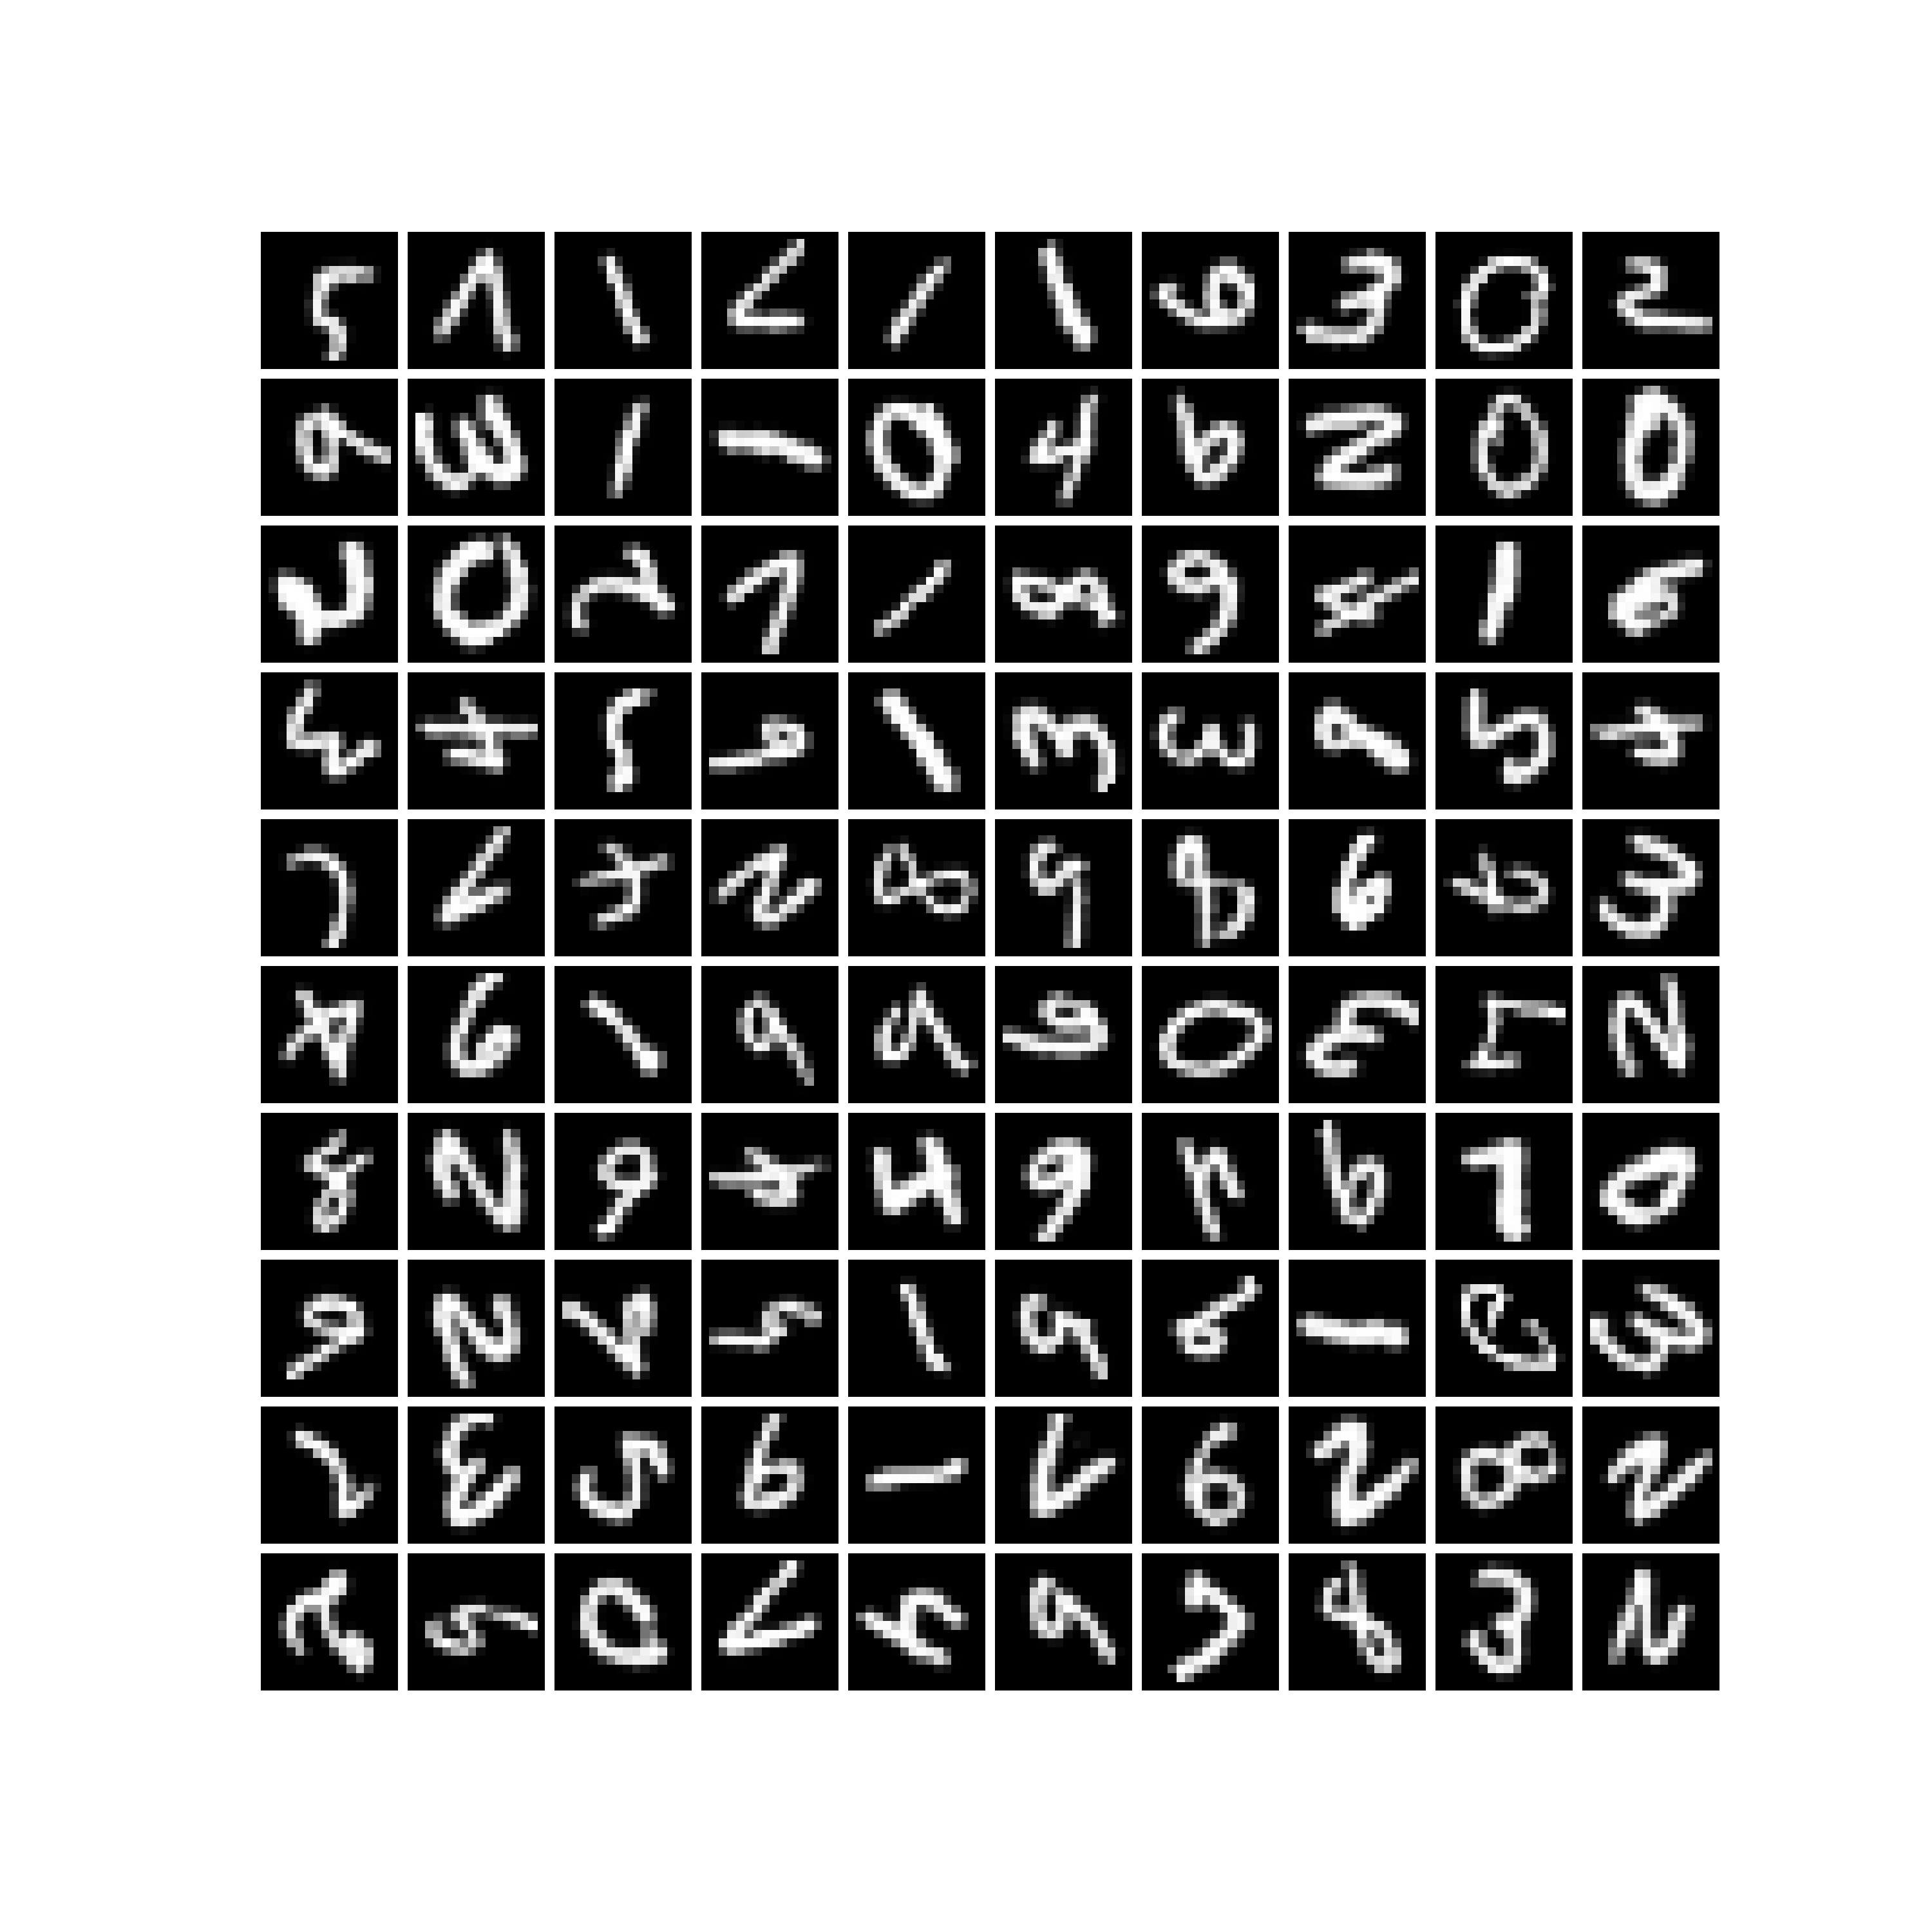
\includegraphics[width=0.4\textwidth]{figs/rotated-mnist.pdf}
%     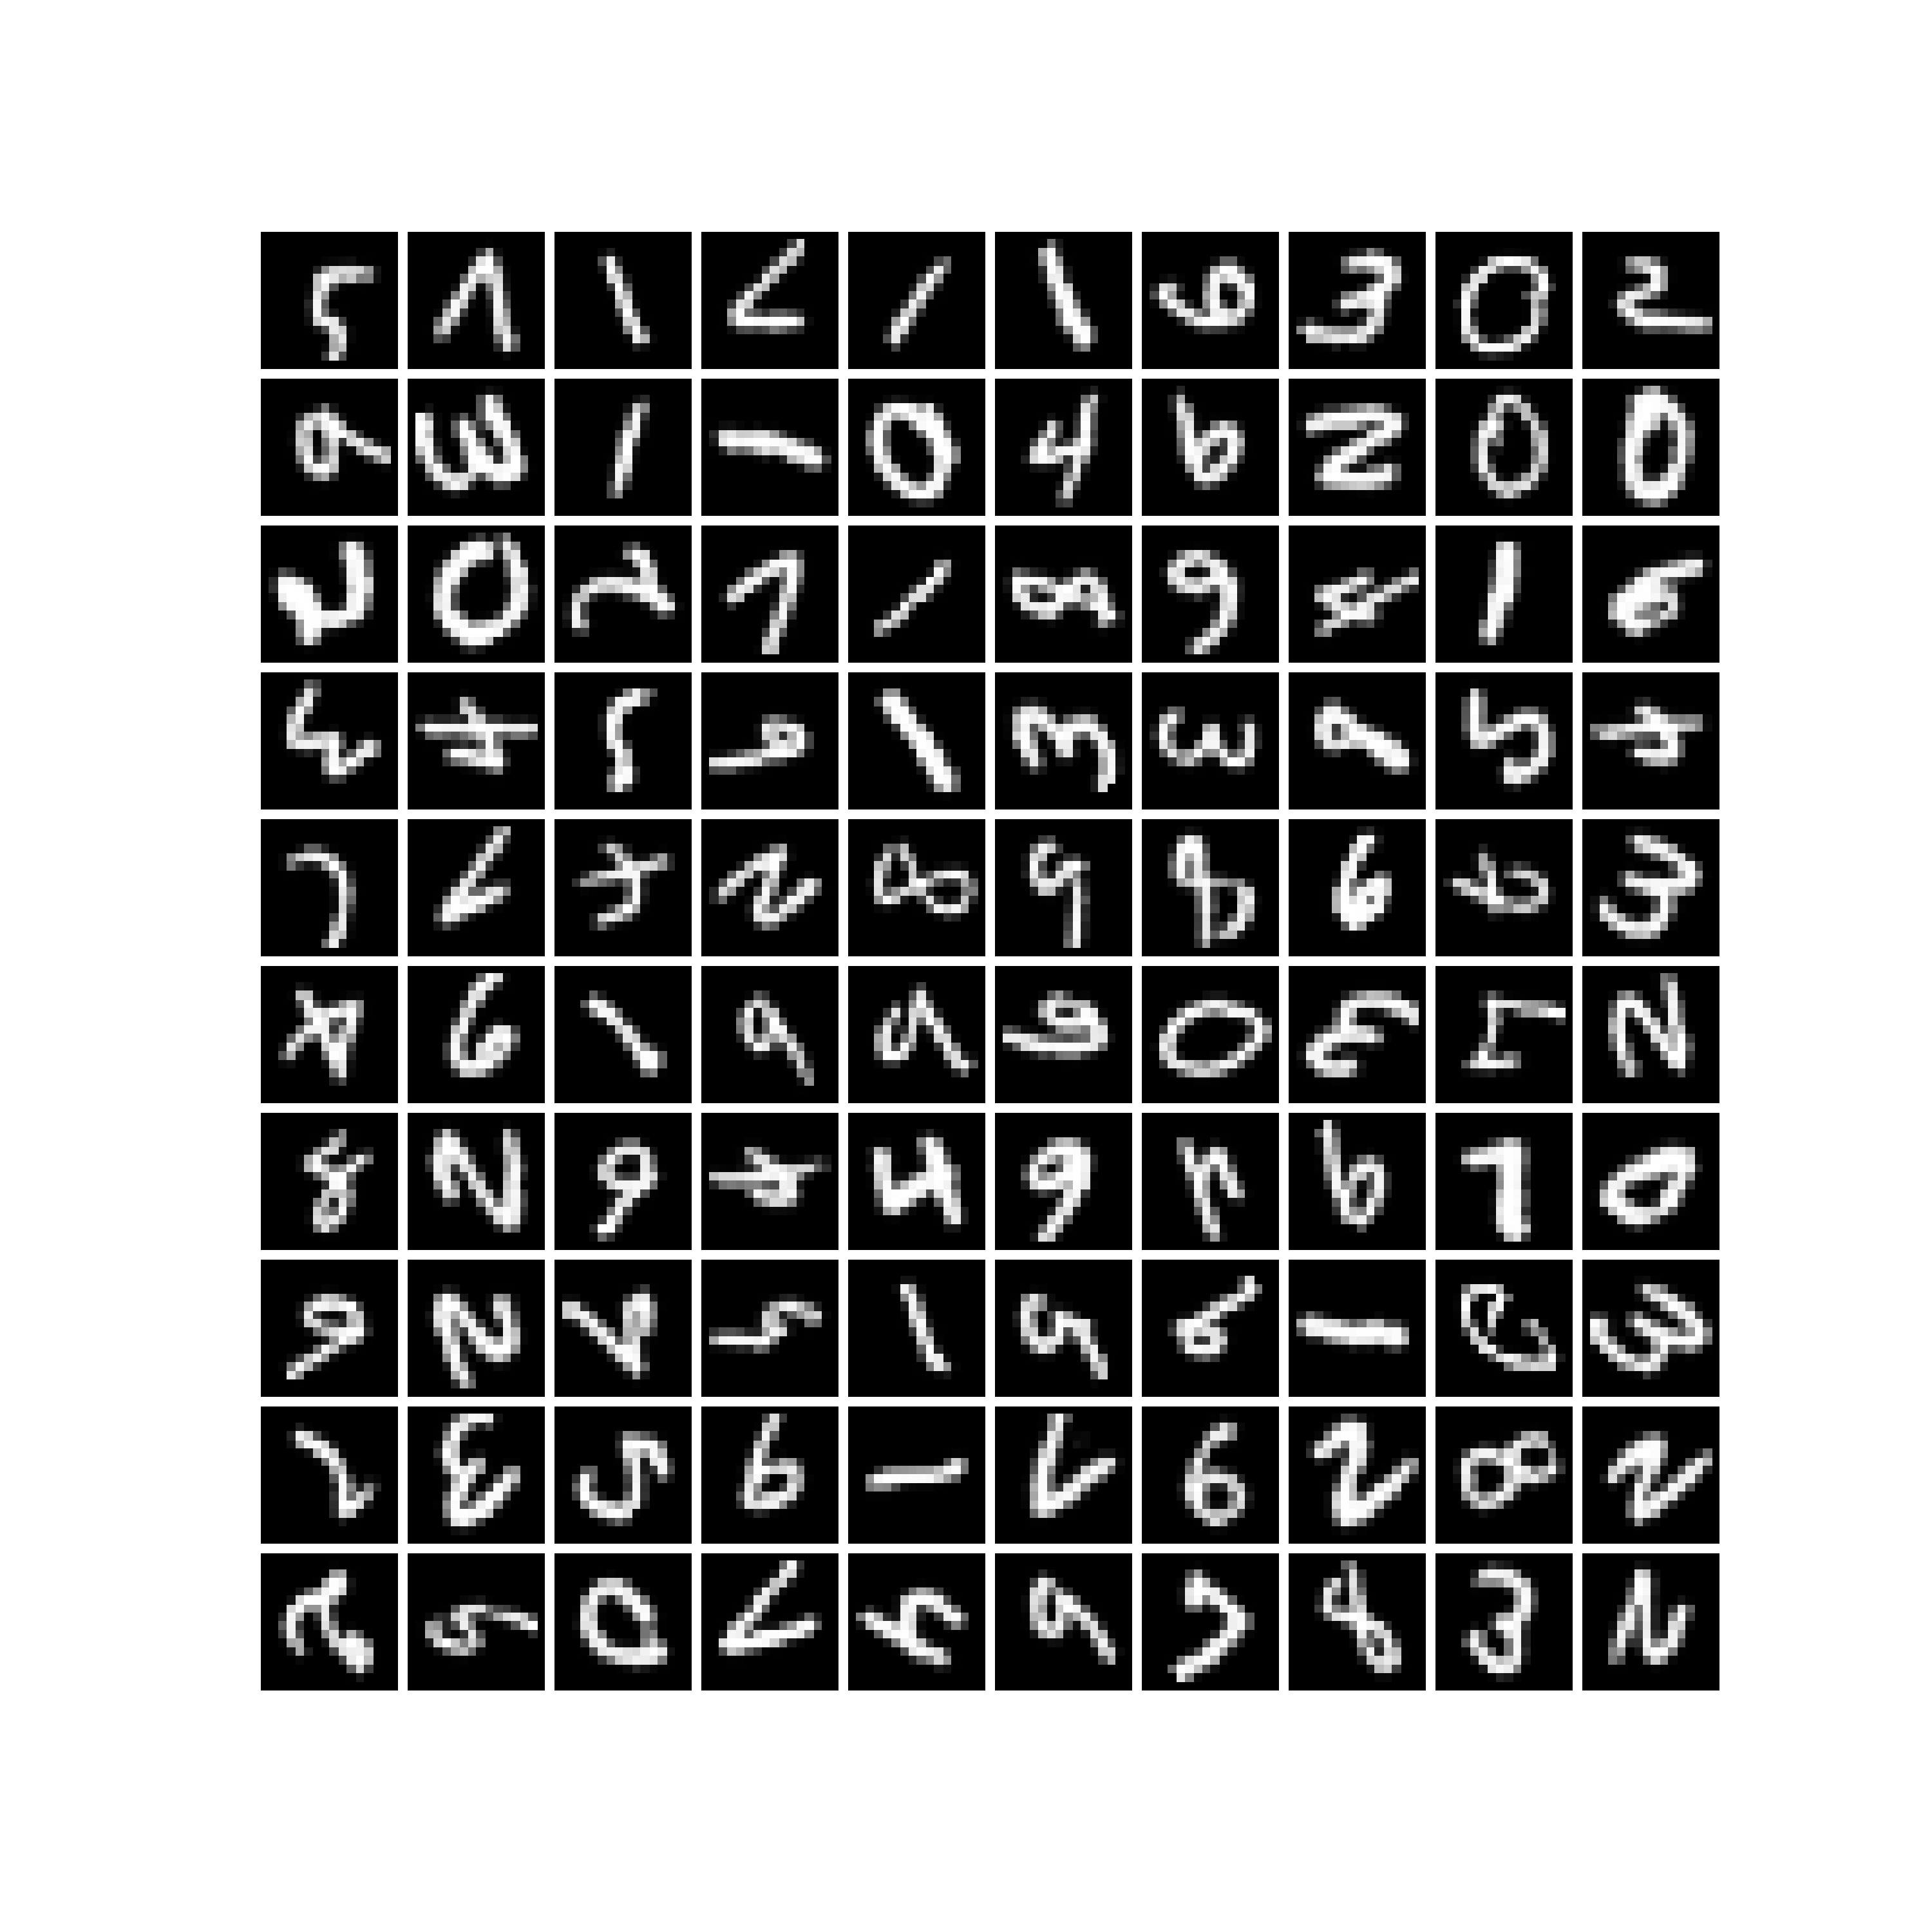
\includegraphics[width=0.4\textwidth]{figs/rotated-mnist.pdf}

%     \caption{Examples from the $SO(2)$-MNIST (left) and $O(2)$-MNIST (right) datasets.}
%     \label{fig:so2-mnist}
% \end{figure}


% \textbf{$O(2)$ MNIST}

% \begin{figure}[H]
%     \centering
%     \includegraphics[width=0.3\textwidth]{example-image-a}
%     \caption{[Figure showing dataset]}
%     \label{fig:o2-mnist}
% \end{figure}

% \textbf{$SE(2)$ MNIST}

% \begin{figure}[H]
%     \centering
%     \includegraphics[width=0.3\textwidth]{example-image-a}
%     \caption{[Figure showing dataset]}
%     \label{fig:se2-mnist}
% \end{figure}


\subsubsection{Models and Training}



\textbf{$C8$-CNN}



\textbf{TC.} The $G$-Conv block consists of an $C8$-Conv block using 24 filters followed by Batch Norm. Next, the $G$-TC Layer is applied. The output is raveled and passed to a three-layer MLP using 1d Batch Norm and ELU nonlinearity and after each linear layer, with all three layers having output dimension $64$. Finally a linear layer is applied, with output dimension $10$, for the 10 object categories.

\textbf{Max.} The $G$-Conv block consists of an $C8$-Conv block using 24 filters followed by Batch Norm and a ReLU nonlinearity. Next, a Max $G$-Pooling Layer is applied. The output is raveled and passed to a three-layer MLP using 1d Batch Norm and ELU nonlinearity and after each linear layer. The first layer has output dimension $275$, to compensate for the difference in output size of the $G$-TC Layer. The remaining two layers having output dimension $64$. Finally a linear layer is applied, with output dimension $10$, for the 10 object categories.

\textbf{$D16$-CNN}

\textbf{TC.} The $G$-Conv block consists of an $D16$-Conv block using 24 filters followed by Batch Norm. Next, the $G$-TC Layer is applied. The output is raveled and passed to a three-layer MLP using 1d Batch Norm and ELU nonlinearity and after each linear layer, with all three layers having output dimension $64$. Finally a linear layer is applied, with output dimension $10$, for the 10 object categories.


\textbf{Max.} The $G$-Conv block consists of an $D16$-Conv block using 24 filters followed by Batch Norm and a ReLU nonlinearity. Next, a Max $G$-Pooling Layer is applied. The output is raveled and passed to a three-layer MLP using 1d Batch Norm and ELU nonlinearity and after each linear layer. The first layer has output dimension $2,380$, to compensate for the difference in output size of the $G$-TC Layer. The remaining two layers having output dimension $64$. Finally a linear layer is applied, with output dimension $10$, for the 10 object categories.


\subsection{ModelNet10 Experiments: $O$ and $O_h$ acting on $\mathbb{R}^3$}

\subsubsection{Datasets}

The ModelNet10 dataset is downsampled and voxelized to a $10 \times 10 \times 10$ grid. for the $O$-ModelNet10 Dataset, each datapoint is transformed by a random cubic rotation. For the $O_h$-ModelNet10 Dataset, each datapoint is transformed by a random cubic rotation and flip. The standard training and testing sets are used. A random $20 \%$ of the training dataset is set aside for model validation and is used to tune hyperparameters. The remaining $80 \%$ is used for training.

% \textbf{$O$ and $O_h$ ModelNet10}

% \begin{figure}[H]
%     \centering
%     \includegraphics[width=0.3\textwidth]{example-image-a}
%     \includegraphics[width=0.3\textwidth]{example-image-a}
%     \caption{[Figure showing dataset]}
%     \label{fig:so3-modelnet}
% \end{figure}



\subsubsection{Models and Training}

\textbf{$O$-CNN}



\textbf{TC}. The $G$-Conv block consists of an $O$-Conv block using 24 filters followed by a IID 3D Batch Norm Layer. Next, the $G$-TC Layer is applied. The output is raveled and passed to a three-layer MLP using 1d Batch Norm and ELU nonlinearity and after each linear layer, with all three layers having output dimension $64$. Finally a linear layer is applied, with output dimension $10$, for the 10 object categories.

\textbf{Max.} The $G$-Conv block consists of an $O$-Conv block using 24 filters followed by a IID 3D Batch Norm Layer and a ReLU nonlinearity. Next, a Max $G$-Pooling Layer is applied. The output is raveled and passed to a three-layer MLP using 1d Batch Norm and ELU nonlinearity and after each linear layer. The first layer has output dimension $5,420$, to compensate for the difference in output size of the $G$-TC Layer. The remaining two layers having output dimension $64$. Finally a linear layer is applied, with output dimension $10$, for the 10 object categories.


\textbf{$O_h$-CNN}





\textbf{TC.} The $G$-Conv block consists of an $O_h$-Conv block using 24 filters followed by a IID 3D Batch Norm Layer. Next, the $G$-TC Layer is applied. The output is raveled and passed to a three-layer MLP, with all three layers having output dimension $64$. Finally a linear layer is applied, with output dimension $10$, for the 10 object categories.



\textbf{Max.} The $G$-Conv block consists of an $O_h$-Conv block using 24 filters followed by a IID 3D Batch Norm Layer and a ReLU nonlinearity. Next, a Max $G$-Pooling Layer is applied. The output is raveled and passed to a three-layer MLP. The first layer has output dimension $20,000$, to compensate for the difference in output size of the $G$-TC Layer. The remaining two layers having output dimension $64$. Finally a linear layer is applied, with output dimension $10$, for the 10 object categories.




% \section{Computing the TC in general cases, and $SE(n)$ in particular}

% \subsection{Are we working with $SE(n)$ or with $SO(n) \tims \mathbb{R}^n$?}

% We first investigate the difference between $SE(n)$ and $SO(n)\times \mathbb{R}^n$ equivariance.

% \paragraph{Group structure}

% The group composition and inverse of the semi-direct product $SE(n) = SO(n) \rtimes \mathbb{R}^n$ are:
% \begin{align*}
%     (R_1, t_1) \cdot (R_2, t_2)
%         &=(R_1.R_2, R_2.t_1+t_2) \\
%     (R, t)^{-1}
%         &= (R^{-1}, -R^{-1}.t).
% \end{align*}

% The group composition and inverse of the direct product $SO(n)\times \mathbb{R}^n$ are:
% \begin{align*}
%     (R_1, t_1) \cdot (R_2, t_2)
%         &=(R_1.R_2, t_1+t_2) \\
%     (R, t)^{-1}
%         &= (R^{-1}, -t).
% \end{align*}

% \paragraph{Action on $\mathbb{R}^n$}
% The group $SE(n)$ acts on $\mathbb{R}^n$ through its so-called homogeneous representation, that converts $(R, t)$ into a matrix.
% \begin{equation}
%     g(R, t) =
%     \begin{pmatrix}
%         R & t \\
%         0 & 1
%     \end{pmatrix}
%     \quad \text{with inverse: }
%         g(R, t)^{-1} =
%         \begin{pmatrix}
%         R^{-1} & -R^{-1}.t \\
%         0 & 1
%     \end{pmatrix}
% \end{equation}
% so that:
% \begin{equation}
%     g^{-1}x = \begin{pmatrix}
%         R^{-1} & -R^{-1}.t \\
%         0 & 1
%     \end{pmatrix} .
%     \begin{pmatrix}
%     x \\
%     1
%     \end{pmatrix}
%     =
%     \begin{pmatrix}
%     R^{-1}x-R^{-1}t \\
%     1
%     \end{pmatrix}
%     =     \begin{pmatrix}
%     R^{-1}(x-t) \\
%     1
%     \end{pmatrix}
% \end{equation}

% By contrast, there is no canonical way of defining the action of the product group $SO(n) \times \mathbb{R}^n$ on $\mathbb{R}^n$. Indeed, if two groups $G_1, G_2$ act on the same space $V$, the standard way of building an action of $G_1 \times G_2$ is to consider the action on the direct sum $V \oplus V$ defined as $(g_1, g_2 \act (x_1, x_2) = (g_1\cdot x_1, g_2 \cdot x_2)$ using two copies of $V$ \footnote{\url{https://math.stackexchange.com/questions/3140677/direct-sum-of-representation-of-product-groups}}. To define the action of $G_1 \times G_2$ on one copy of $V$, we can choose which group acts first and get:
% \begin{align*}
%     (R, t) \cdot x
%         &= (Rx + t)
%         \quad \text{(Choice 1: applying $R$ first and then $t$)},\\
%     (R, t) \cdot x
%         &= R(x+t)
%         \quad \text{(Choice 2: applying $t$ first and then $R$)}.
% \end{align*}
% which we compare to the action of $SE(n)$:
% \begin{equation}
%     (R, t) \cdot x = Rx + t.
% \end{equation}
% Both $SO(n) \times \mathbb{R}^n$ (Choice 1) and $SE(n)$ consider that we first apply the rotation, and then translate.

% The application of $(R^{-1}, -t)$ gives:
% \begin{align*}
%     (R^{-1}, -t) \cdot x
%         &= (R^{-1}x - t)
%         \quad \text{(Choice 1)},\\
%     (R^{-1}, -t)\cdot x
%         &= R^{-1}(x-t)
%          \quad \text{(Choice 2)}.
% \end{align*}
% which we compare to the action of $SE(n)$:
% \begin{equation}
%     (R, t)^{-1} \cdot x  =R^{-1}(x-t)
% \end{equation}
% Both $SO(n) \times \mathbb{R}^n$ (Choice 2) and $SE(n)$ will yield the definition of convolution from \cite{cesa2021program}.

% Consequently, the action of $SE(n)$ on $\mathbb{R}^n$ is a mix of the action of $SO(n) \times \mathbb{R}^n$ (choice 1) and of $SO(n) \times \mathbb{R}^n$ (choice 2).


% \paragraph{Group-convolution} The group convolution using the semi-direct product $SE(n) = SO(n) \ltimes \mathbb{R}^n$ writes:
% \begin{align*}
%     \Theta(g)
%     = (f \ast \phi)(g)
%     =\int_{x \in \mathbb{R}^n} f(x)\phi(g^{-1}x)dx.
% \end{align*}
% and only uses the composition by an inverse element $g^{-1}x$. Thus, it can be the inverse in the $SE(n)$ setting or in the $SO(n) \times \mathbb{R}^2$ (Choice 2):
% \begin{align*}
%     \Theta(g)
%     = (f \ast \phi)(g)
%     =\int_{x \in \mathbb{R}^n} f(x)\phi(g^{-1}x)dx
%     =\int_{x \in \mathbb{R}^n} f(x)\phi(R^{-1}(x-t))dx
% \end{align*}
% which is equation (1) in \cite{cesa2021program}.

% \paragraph{Conclusion} In \cite{cesa2021program}, the authors state: ``We focus on convolutional networks on Euclidean spaces X = Rn, acted on by the group $(\mathbb{R}^n, +) \rtimes G$, i.e. the semidirect product of translations in $(\mathbb{R}^n, +)$ and origin-preserving transformations $G \leq O(n)$``. Both the words "semi-direct product" and "origin-preserving transformations" seems to indicate that we use $SE(n)$. This is because, when we first rotate and then translate, then the rotation is always preserving the origin of the domain. Additionally, in \cite{cohen2016group}, they say: ``The group p4 acts on points in Z2 (pixel coordinates) by multiplying the matrix g(r, u, v) by the homogeneous coordinate vector x(u′, v′) of a point (u′, v′)``, which corresponds indeed to the action of $SE(n)$.


% \subsection{Compute TC with escnn's API for any group $G \ltimes \mathbb{R}^n$}

% We provide the full computations for the special cases $SE(2) = SO(2) \ltimes \mathbb{R}^2$ and $E(2) = O(2) \ltimes \mathbb{R}^2$, and then extract a general strategy for any group $G \ltimes \mathbb{R}^n$.

% \paragraph{TC with $SE(2)$ in practice} Elements of $SE(2)$ will be indexed by $(r, u, v)$ where $r$ is the angle of the 2D rotation and $u, v$ represent the 2D translation.

% We recall that for $SE(2) = SO(2) \ltimes \mathbb{R}^2$. The output of the $SO(2)$-steerable convolution (i.e. of the $SE(2)$ convolution) is of shape $C_\text{out}|G| \times W \times H$. Consequently, reshape into $C_\text{out} \times |G| \times W \times H$ ad denote $r$ the index going though the group indices and $u, v$ the indices going through the domain indices.

% To find the element $\Theta(gg_i)$ needed for the TC, we need to find the indices $(r, u, v)$ that correspond to the product of two group elements $(r_1, u_1, v_1)$ and $(r_2, u_2, v_2)$. We can then use $g = g_1$ and $g_i = g_2$ to get the result.

% As \texttt{escnn} only thinks in terms of $G$ within $G \ltimes \mathbb{R}^2$, they do not have a group Python class dedicated to $SE(2)$. Thus, we need to implement the group composition of $SE(2)$ manually.

% We have the following correspondence between indices and matrices:
% \begin{equation}
%     (r, u, v)
%     &=
%     \begin{pmatrix}
%         R_2 & t_2 \\
%         0 & 1
%     \end{pmatrix}
%     &=
%     \begin{pmatrix}
%     \cos(r\pi/2) & -\sin(r\pi/2) & u \\
%     \sin(r\pi/2) & \cos(r\pi/2) & v \\
%     0 & 0 & 1
%      \end{pmatrix}
% \end{equation}

% So that the group composition written in indices, can be computed as:
% \begin{align*}
%     (r_1, u_1, v_1) \cdot (r_2, u_2, v_2)
%     &=     \begin{pmatrix}
%         R_1 & t_1 \\
%         0 & 1
%     \end{pmatrix} .
%         \begin{pmatrix}
%         R_2 & t_2 \\
%         0 & 1
%     \end{pmatrix} \\
%     &=
%     \begin{pmatrix}
%         R_1.R2 & R_1.t_2+t_1 \\
%         0 & 1
%     \end{pmatrix} \\
%     &=
%     \begin{pmatrix}
%     \cos((r_1+r_1)\pi/2) & -\sin((r_1+r_1)\pi/2) & u \\
%     \sin((r_1+r_1)\pi/2) & \cos((r_1+r_1)\pi/2) & v \\
%     0 & 0 & 1
%      \end{pmatrix},
% \end{align*}
% where the elements of the resulting translations are:
% \begin{align*}
%     u &= \cos(r_1\pi/2)u_2 -\sin(r_1\pi/2)v_2 \\
%     v &= \sin(r_1\pi/2)u_2 -\sin(r_1\pi/2)v_2.
% \end{align*}
% Now, we need to find the (integer) indices to which $u, v$ correspond to. This can be approximated by $u \leftarrow int(u)$ and $v \leftarrow int(v)$ where int means integer. Consequently, the group composition formula is, in terms of indices:
% \begin{align*}
%     &(r_1, u_1, v_1) \cdot (r_2, u_2, v_2)\\
%     &= (r_1 + r_2, int(\cos(r_1\pi/2)u_2 -\sin(r_1\pi/2)v_2), int(\sin(r_1\pi/2)u_2 -\sin(r_1\pi/2)v_2).
% \end{align*}

% \paragraph{TC with $SE(2)$ in code}
% We convert this formula into pseudo-code that uses \texttt{escnn}'s API, assuming that CN is the cyclic group that discretizes the rotations in $SE(2)$.
% \begin{align*}
%     (r_1, u_1, v_1) \cdot (r_2, u_2, v_2) = (r, u, v)
% \end{align*}
% where:
% \begin{align*}
%     r &= CN.\_combine(r_1, r_2) \\
%     u &= int(CN.\_change\_param(element=r_1, p\_from="int", p\_to="MAT") @ [u_2, v_2])[0] \\
%     v &= int(CN.\_change\_param(element=r_1, p\_from="int", p\_to="MAT") @ [u_2, v_2])[1].
% \end{align*}
% We use $\Theta(r, u, v)$ (at indices $r, u, v$) to get $\Theta(g_1.g_2).$

% \paragraph{TC with $E(2)$ in code} We can generalize this to $E(2)$ by considering the DN dihedral group:
% \begin{align*}
%     (m_1, r_1, u_1, v_1) \cdot (m_2, r_2, u_2, v_2)= (m, r, u, v)
% \end{align*}
% where:
% \begin{align*}
%     (m, r) &= DN.\_combine((m_1, r_1, m_2, r_2))\\
%     u = &= int(CN.\_change\_param(element=(m_1, r_1), p\_from="int", p\_to="MAT") @ [u_2, v_2])[0]\\
%     v= &= int(CN.\_change\_param(element=(m_1, r_1), p\_from="int", p\_to="MAT") @ [u_2, v_2])[1].
% \end{align*}

% \paragraph{TC with any $SE(n) \ltimes \mathbb{R}^n$ or $G \ltimes \mathbb{R}^n$ in code}. The above strategy can be applied to any $G \ltimes \mathbb{R}^n$ where $G$ is a group implemented in escnn/group/groups, as it only requires the use of combine (for the $G$-part) and change-param (for the $\mathbb{R}^n$-part). In particular, it applies to any $SE(n) = SO(n) \ltimes \mathbb{R}^n$.

% For general $G$ and for $SO(3)$, in order to use the change-param function to convert the 3D rotation into a MAT, we need to know what param is used to represent elements at the output of the G-conv. For example, the possible params for $SO(3)$ are given in \url{https://github.com/QUVA-Lab/escnn/blob/master/escnn/group/groups/so3_utils.py}.


% \textbf{$SE(3)$-CNN}

% \textit{Max}

% \textit{TC}
